% Class options:
% - Use `noindent` for a non-indented version of the report
% - Use `public` to mark the document for public use
% - Use `restricted` to mark the document for internal use only
% - Use `confidential` to mark the document as confidential
% - Use `strictlyconfidential` to mark the document as strictly confidential
% For more details, see https://intern.aisec.fraunhofer.de/display/ISMS/Informationsklassifizierung
% and https://ocs.zv.fraunhofer.de/OTCS/livelink.exe/open/408035
\documentclass[strictlyconfidential,noindent]{aisecreport}

\usepackage[ngerman, english]{babel}

\usepackage{listings}
\lstdefinestyle{shell}{
    language=bash,
    basicstyle=\footnotesize\ttfamily, 
    keywordstyle=\color{blue}, 
    commentstyle=\color{green!50!black}, 
    stringstyle=\color{red}, 
    showstringspaces=false, 
    tabsize=2,
    frame=single, 
}
\usepackage[backref=true]{biblatex}
\addbibresource{document.bib}
\usepackage{graphicx}
\usepackage{subcaption}


% Draft mode
% \usepackage{draftwatermark}
% \SetWatermarkAngle{45}
% \SetWatermarkLightness{0.9}
% \SetWatermarkFontSize{5cm}
% \SetWatermarkScale{1}
% \SetWatermarkText{DRAFT}

% Commands for TODOs, FIXMEs, and other notes
\usepackage{xcolor}
\newcommand{\todo}[1]{{\color{red}\textbf{TODO(}}{\color{white!25!black}#1}{\color{red}\textbf{)}}}
\newcommand{\fixme}[1]{{\color{blue}\textbf{FIXME(}}{\color{white!25!black}#1}{\color{blue}\textbf{)}}}
\newcommand{\note}[1]{{\color{green!50!black}\textbf{NOTE(}}{\color{white!25!black}#1}{\color{green!50!black}\textbf{)}}}

\title{IDP: Post-Quantum Cryptography in Unikernels}
\subtitle{Evaluating Post-Quantum Cryptography in Unikernels on Embedded Devices}
% \version{0.1}

\author{
    Moritz Beckel
}
\date{\today}

\begin{document}

\uppertitleback{}
\lowertitleback{
	\begin{flushleft}
	Fraunhofer Research Institution for Applied and Integrated Security\\
	\url{www.aisec.fraunhofer.de}\\[5mm]
	Fraunhofer AISEC\\
	Lichtenbergstraße 11\\
	85748 Garching (near Munich)\\
	Germany\\[5mm]
	Contact: Moritz Beckel \\
	\texttt{moritz.beckel@tum.de}
	\end{flushleft}
}

\maketitle
\tableofcontents

%%
\chapter{Motivation}

With Harvest-Now-Decrypt-Later attacks, quantum computing already creates vulnerabilities in today's systems, and with increasing research on quantum computing, other attacks might soon become feasible against classical cryptography. Fortunately, post-quantum cryptography already exists, and it works with new mathematical problems that are not efficiently solvable by quantum computers. Post-quantum cryptography has already found its way into major network protocols such as Transport Layer Security (TLS) with algorithms that perform similarly or even better than former insecure ones. TLS is one of the most critical security protocols, not only used by personal and enterprise computers but also by embedded devices. In recent years, software-based isolation has become a major topic in embedded software. Currently, the most prominent solution for isolation is containerization. However, container solutions often depend on a full-fledged operating system as a host, which is not suitable for low-performance embedded devices. An alternative solution is unikernels, which run fully virtualized on a hypervisor and instead reduce overhead by excluding unnecessary operating system parts. Because of different software architecture, the performance often deviates even when the same user space application is run. As TLS is a vital protocol to any operating system, a small difference in performance can have a major impact on the usability of the system. Because post-quantum cryptography is inherently different, there is a strong possibility that their performance also differs when run on a unikernel, and for this reason, post-quantum cryptography is to be evaluated in the context of a unikernel.

This Interdisciplinary Project revolves around integrating the post-quantum cryptography library liboqs into the Unikraft unikernel and comparing several performance metrics to a native solution and a containerized solution. 

Our first task was to evaluate the hardware at hand and choose a platform comparable to industry standards. We chose a Raspberry Pi 4B model, as it has wide development support and is ARM-based, making it more comparable to low-powered industrial hardware.

Our second task was to define use cases that will be used as a basis for the evaluation. Since one of post-quantum cryptography's use cases is TLS, and TLS is one of the most widely used network protocols, we opt for benchmarking the performance of network connections via TLS/HTTPS. 

Our third task was to define measurands and evaluate the performance of a unikernel with post-quantum cryptography. We measure the networking performance with TLS by the number of TLS connections per second, and we measure the runtime of post-quantum cryptography primitives. During which we also take a look at the overall power consumption and memory allocation.
Finally, we evaluate the usability of the system by means of build time, toolchain complexity, etc. To solve this task, we built a test setup in this repository, which contains a configuration for a Unikraft unikernel capable of post-quantum cryptographic primitives and a new OpenSSL version that can make use of those primitives. For comparison, the repository also contains configurations for a Docker Container and a native setup that have the same solution running. 


%%
\chapter{Background}
\label{chapter:background}

In this section, we present the necessary background information to fully grasp the impact of Post-Quantum Cryptography on current cryptography standards. Specifically, the changes that need to be made to a TLS implementation (e.g., OpenSSL), so we can no longer break the protocol with sufficient computing power. We then introduce the notion of a unikernel as an alternative virtualization method to containers. 

\section{TLS Protocol}

\begin{figure}
    \centering
    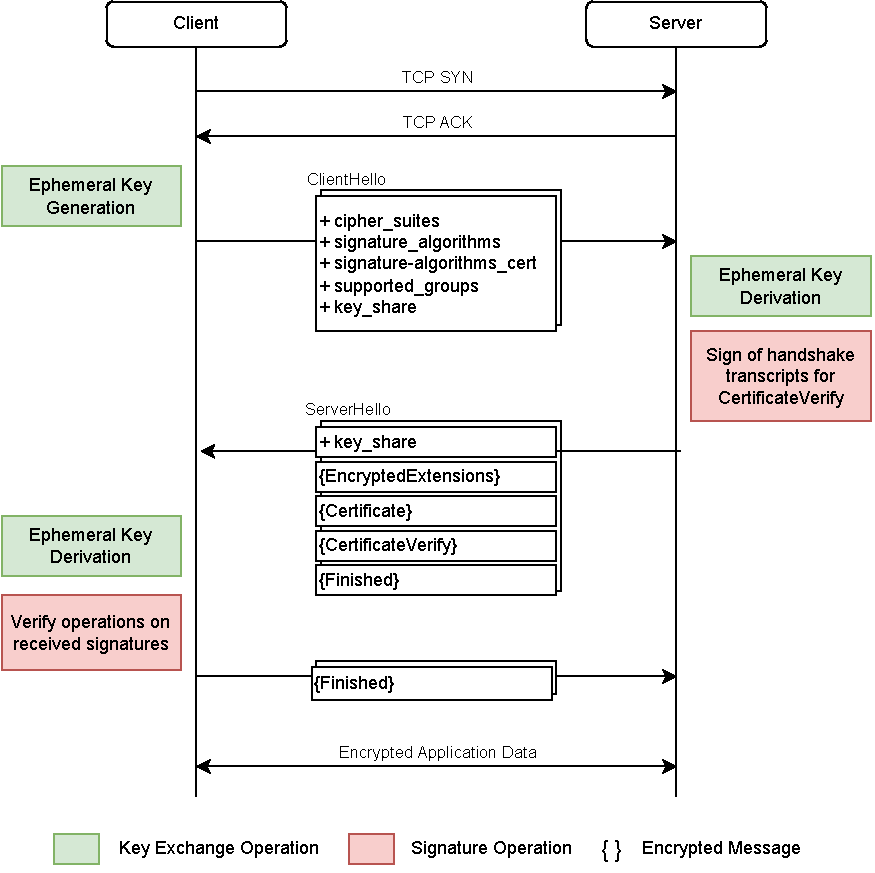
\includegraphics[width=0.5\textwidth]{resources/tls_overview.pdf}
    \caption{TLS 1.3 Handshake Overview.}
    \label{fig:tls_handshake}
\end{figure}

TLS is a network protocol that works on top of the TCP protocol. Its main goal is to ensure confidentiality, authenticity, and integrity. We now examine the basic principle of TLS and single out those cryptographic operations that are not strong enough to withstand a post-quantum attack and need to be replaced by newer PQC. We will do so by observing a typical connection establishment of the TLS 1.3 protocol, which is defined in \cite{rescorla2018transport}. As TLS is an extensive protocol with many extensions, we examine a connection where only the server authenticates itself, and the server and client do not have any pre-shared keys. A graphical overview of the TLS handshake is presented in Figure \ref{fig:tls_handshake}.

The TLS handshake starts once a TCP handshake is done and establishes a stateful connection. It begins by sending a \textit{ClientHello} message, which contains several attribute fields. We omit most fields and only focus on the ones important for encryption. The first encryption-related field is the \textit{cipher\_suites} field, which contains a list of \textbf{symmetric ciphers} that the client supports. The next two fields are the \textit{signature\_algorithms} and \textit{signature\_algorithms\_cert} fields that contain digital signature algorithms supported by the client. The final two fields are the \textit{supported\_groups} and \textit{key\_share} fields. These include all supported \textbf{key exchange algorithms} and the corresponding key material, which is used to share a secret key that both client and server can use for symmetric encryption. Upon receiving the message, the server selects a key exchange algorithm from the list of supported groups and calculates the shared secret.

The server responds with a \textit{ServerHello} message that contains the \textit{key\_share} field with its own key material so that the client can deduce the shared secret as well. The message also contains the selected algorithm for symmetric encryption in the \textit{cipher\_suite} field. Afterwards, the server sends the \textit{EncryptedExtensions} message that contains additional extensions (e.g., the TCP segment size). Next, the server authenticates itself by sending the \textit{Certificate} message that contains the server's certificate chain and the \textit{CertificateVerify} message, which shows that the previous messages were exchanged with the server. The server does so by calculating a \textbf{hash} over the handshake context and the certificate chain and then calculating a \textbf{digital signature} over the hash with the server's private key. The client then verifies the digital signature with the server's public key, and the client verifies the public key (contained in the server's certificate) by going up the certificate chain and comparing the top with the client's own root certificate. The last two messages are the \textit{Finished} messages, which both the client and the server send. They signal that neither server nor client has anything further to add to the handshake, and they contain a \textbf{Message Authentication Code (MAC)} of the entire handshake to ensure nothing was omitted. Once the \textit{Finished} messages are exchanged, the TLS connection is established, and it is now possible to exchange user data. From now on, the shared secret is used for encryption, for both user data and status messages of the TLS protocol. 

We can see that TLS makes use of several cryptographic operations: symmetric encryption, key exchange algorithms, digital signatures, hash functions, and MACs. As examined by Chen et al. \cite{chen2016report}, we can see that multiple operations are susceptible to quantum-capable attackers:  Classical key exchange algorithms are based on the Diffie-Hellman algorithm, which uses the discrete logarithm problem for security \cite{maurer2000diffie}. However, with Shor's Algorithm, quantum computers can solve this problem in polynomial time, making it insecure \cite{shor1999polynomial}. The same goes for digital signatures that typically use ECDSA and RSA algorithms, which are again based on the discrete logarithm problem or the integer factorization problem, that are weak against quantum computers \cite{mahto2017rsa, shor1999polynomial}. For symmetric encryption, the impact is not as drastic, as no efficient solution to the underlying problems has been found yet. Though Grover \cite{grover1996fast} discovered that it is possible to speed up general search algorithms quadratically with quantum computers, which means that we can also search faster for a symmetric key. However, if we double the key size, we can maintain the same security as before. The same applies to hash functions \cite{alnahawi2024comprehensive}. They are also considered secure, given that they have a larger output. Message authentication codes are based either on symmetric ciphers or hash functions, which means they are also considered as secure as symmetric encryption or hashing \cite{bhaumik2024committing}. An overview of the different cryptographic operations and their security is shown in TABLE \ref{tab:ops_security}. Fortunately, we can see that vulnerable operations are primarily used in the handshake, as later everything is symmetrically encrypted with the shared secret, and they are limited to key exchange and digital signatures, which means we have to find alternatives for key exchange and digital signature algorithms. 

\begin{table}[h]
    \centering
    \begin{tabular}{|c|c|c|}
        \hline
        \textbf{Operation} & \textbf{Example Algorithm} & \textbf{Quantum-Resistance} \\
        \hline
        Symmetric Cipher & AES128 & Requires larger keys \\
        %\hline
        Hash Function & SHA256 & Requires larger output  \\
        %\hline
        MAC & HMAC & Requires larger output \\
        \hline
        Public Key Cipher & RSA-2048 & Insecure \\
        %\hline
        Digital Signature & RSA-2048 & Insecure \\
        %\hline
        Key Exchange & ECDHE & Insecure \\
        \hline
    \end{tabular}
    \caption{Resistance of Classical Cryptography to Quantum-Based Attacks \cite{chen2016report}}
    \label{tab:ops_security}
\end{table}

Key exchange algorithms need to be migrated immediately because of the possibility of a Harvest-Now-Decrypt-Later attack, wherein an adversary that is on-path can eavesdrop and store messages, and once quantum computers are powerful enough to break key exchange algorithms, the adversary can use them to recover the shared secret and decrypt all messages of the entire session. This attack requires an adversary to store a session from the beginning and acquire the key material from the TLS handshake, as this is the point where the TLS protocol is most vulnerable. 

Authentication via certificates is less of a problem for current TLS connections: Adversaries can impersonate a peer by breaking its keypair and issuing false certificates before the lifetime of the keypair ends. This attack also depends on the TLS handshake at the beginning of a TLS session. However, an adversary needs to actively participate in the connection, impersonate a peer, and only perform the attack while the session is ongoing, meaning it is not possible to perform this attack as long as we do not have a powerful enough quantum computer. Nevertheless, early adoption is still important as authentication with certificates is based on chaining with global root certificates on top of the chain having a life span of 20 years \cite{ietf-uta-pqc-app-00}. This means that if quantum-based attacks become feasible in this time span, root certificates that are trusted by and stored on the majority of devices need to be removed.

\section{Post-Quantum Cryptography}

In the previous section, we showed how the TLS protocol works and what cryptographic operations it uses. In this section, we examine different key exchange algorithms regarding security and efficiency. We focus mainly on algorithms that have been standardized, as they are the most likely to be considered for implementation in libraries such as OpenSSL. 

The National Institute of Standards and Technology (NIST) is the most well-known entity that tries to agree on common ciphers that will be later implemented in network protocols such as TLS. Starting in 2016, NIST held a competition to find suitable PQC ciphers. In several rounds \cite{moody2019status, alagic2020status, alagic2022status, alagic2025status}, ciphers were submitted and analyzed for weaknesses. Forty ciphers have been included, and a select few were standardized over the course of 6 years. NIST publishes them as a Federal Information Processing Standard (FIPS). Currently, three have been published \cite{unknown-author-2024, unknown-author-2024-2, unknown-author-2024-3} and two more have already been announced \cite{boutin-2025-2, Boutin_2025}. NIST also specifies five security levels for the proposed ciphers \cite{national2016submission}. The levels resemble the difficulty it takes to break the cipher in ascending order, and the difficulty is specified by comparing the cipher to symmetric cryptography, i.e., AES, and SHA. Starting with the first level, an adversary should require the same computational resources needed to break AES128 (SHA256, AES192, SHA384, AES256 with higher levels). Apart from NIST, other institutions are also trying to standardize PQC, mainly the International Standardization Organization (ISO), which includes other algorithms that NIST has not chosen \cite{ISO86890}. 

\section{Exchanging Keys with Post Quantum Cryptography}

At the moment, all institutions propose PQC suitable methods for exchanging keys. Instead of a Diffie-Hellman-based key exchange, all institutions agree on the use of the Key Encapsulation Mechanism (KEM) \cite{fipskem}: During a key exchange between a server and a client, the client first sends its public key. The server then encapsulates a shared key by encrypting a randomly-chosen secret with the client's public key. The server then sends it back to the client. The client decapsulates the shared key by decrypting the ciphertext with the private key. As KEM works very similarly to Diffie-Hellman, no changes in the TLS protocol flow need to be made in order to use it; however, KEM is not forward secure by default because it reuses the key pair. To achieve forward secrecy, the key pair needs to be regenerated for each connection \cite{sfluhrer-cfrg-ml-kem-security-considerations-03}. 

We now examine ciphers that are being recommended by the institutions mentioned above. We compare security, performance, and power consumption. Security is defined by the underlying mathematical problem (e.g., integer factorization) and by the ciphertext indistinguishability property that formally verifies the security of a cryptosystem given that the previous mathematical problem holds. For ciphertext indistinguishability, NIST suggests Indistinguishability under adaptive chosen-ciphertext (IND-CCA2) \cite{alagic2022status}. Classifying the mathematical problems is not as simple because they inherently differ and require deep knowledge to do a proper comparison. Furthermore, there is no proof of hardness for these problems. They are only considered secure so long as no efficient solution has been found, which generally means the older a problem is, the more secure it is considered. For this reason, we only consider the recency of a used mathematical problem. 
For performance, we compare the execution time to Elliptic-Curve based Diffie-Hellman (ECDHE) in a TLS 1.3 handshake. We chose ECDHE as it is currently a supported algorithm in the TLS 1.3 standard and is widely used for comparison in other work. We show the relative runtime overhead (e.g., 1.5x times higher execution time). Finally, we show the relative overhead for power consumption (e.g., 1.5x times higher power consumption):

\textbf{Kyber} (also called ML-KEM) was specified in FIPS 203 \cite{unknown-author-2024-3} and is currently the first choice for KEM ciphers. It is based on the Module-Learning-With-Error, a more recent specialization of a lattice problem, and currently has IND-CCA2 hardness \cite{avanzi2019crystals}. Performance-wise, it is the best among lattice-based ciphers, and it is comparable to a classical key exchange with ECDHE for NIST level 1 when used in TLS 1.3, and for higher levels, Kyber can even outperform ECDHE \cite{doring2022post}. Kyber also has similar power consumption in TLS 1.3 when compared to ECDHE \cite{tasopoulos2023energy}.

\textbf{HQC} was chosen to be standardized as an alternative to Kyber by NIST because of the different underlying mathematical problem \cite{Boutin_2025}. A standardization draft is expected to be released in 2026. It is based on the Quasi-Cyclic Syndrome Decoding problem, which is a specialization of a code-based problem and also has IND-CCA2 hardness \cite{gaborit2025hamming}. Performance-wise, it is the best among code-based ciphers. On NIST level 1, HQC has a slight overhead of 1.45x - 1.8x when compared against ECDHE \cite{sikeridis2020assessing, alnahawi2024comprehensive}. HQC's power consumption is double that of ECDHE\cite{tasopoulos2023energy}.

Additionally, NIST also lists other ciphers which still have not been disqualified but have not been chosen for standardization so far, including: Saber, NTRU and NTRU Prime, Classic McEliece, BIKE, and FrodoKEM \cite{alagic2022status, alagic2025status}. Most are not preferred either because of worse performance or stronger hardness assumptions of the ciphertext indistinguishability property. So far, they have been listed as alternative algorithms by NIST and are still being improved, so they remain an option if a cipher chosen for standardization is broken. A subset of alternative ciphers is also included in other standards: 

\textbf{FrodoKEM} was specified in ISO 18033-2 \cite{ISO86890} and is also recommended by BSI \cite{unknown-author-2024-4}. ISO considers it a conservative choice over Kyber as it uses the unmodified and well-studied Learning-With-Errors problem instead of the modified version used by Kyber \cite{unknown-author-2024-4, FrodoKEM2024}. It has IND-CCA2 hardness. FrodoKEM comes in two variants: FrodoKEM-AES and FrodoKEM-SHAKE, which use either AES or SHAKE to generate a large parameter matrix A for later use in the algorithm. While FrodoKEM-SHAKE generally performs better, FrodoKEM-AES has the advantage that AES can be hardware accelerated \cite{NIST-FrodoKEM-20200930}. On average, its performance overhead on NIST level 1 is 2.5x when compared with ECDHE \cite{alnahawi2024comprehensive}. FrodoKEM's Power consumption is roughly 14x times that of ECDHE \cite{tasopoulos2023energy}.

\textbf{BIKE} was part of all standardization rounds until the fourth round \cite{alagic2025status}. It is based on the Quasi-Cyclic Moderate Density Parity-Check problem, which is a code problem, and it has IND-CCA2 hardness. On average, its performance overhead on NIST level 1 is 2.55 when compared to ECDHE \cite{alnahawi2024comprehensive}. BIKES's Power consumption is roughly 8 times that of ECDHE \cite{tasopoulos2023energy}. 

NIST's choices perform similarly to old key exchange ciphers. However, their underlying mathematical problems are still relatively new and not as field-tested. On the other hand, ISO's choices rely on older, well-studied mathematical problems, which are less likely to be broken, but at the same time, they have a higher overhead. Fortunately, this overhead is manageable even on weaker hardware, e.g., it was shown by \cite{wagner-2025} that it is possible to implement even Classic McEliece with its large key sizes on an embedded system. Now, adversaries still have the ability to spoof an active connection by issuing false certificates, which is why we also need to make use of post-quantum digital signatures.

\section{Providing Certificates with Post Quantum Cryptography}

Just like we did with key exchange algorithms, we examine different digital signature algorithms in terms of security and efficiency, and we will focus on ciphers that have been standardized. Functionally, post-quantum digital signatures behave exactly as classical signatures, which means they can act as a drop-in replacement in the TLS protocol. Again, we analyze security, efficiency, and power consumption, and we compare the signature algorithms to the Elliptic-Curve-based Digital Signature Algorithm (ECDSA) in a TLS 1.3 handshake. ECDSA is currently a supported algorithm in the TLS 1.3 standard and is widely used for comparison in other work. We show the relative overhead of the execution time and the power consumption (e.g., 1.2x times higher execution time). For security of the cryptosystem, NIST suggests Existential Unforgeability under Chosen Message Attack (EUF-CMA) \cite{national2016submission}.

\textbf{Dilithium} (also called ML-DSA) was specified in FIPS 204 \cite{unknown-author-2024} and is currently the first choice for post-quantum digital signatures. It makes use of the Module-Learning-With-Error and Module-Short-Integer-Solution problems, which are based on the lattice problem \cite{CRYSTALSDIL}. Its hardness is Strong Existential Unforgeability under Chosen Message Attack and meets the requirements of NIST \cite{CRYSTALSDIL, national2016submission}. The performance of Dilithium is comparable to classical ECDSA, and its power consumption is also comparable \cite{doring2022post, tasopoulos2023energy}.

\textbf{FALCON} (also called FN-DSA) was chosen to be standardized by NIST as an alternative algorithm to Dilithium with similar performance \cite{boutin-2025-2}. A standardization draft is expected to be released in 2026. It makes use of the NTRU problem, which is based on the lattice problem \cite{fouque2020falcon, alnahawi2024comprehensive}. Falcon's hardness is proof of unforgeability in the QROM, which is deemed to be comparable to Dilithium \cite{boneh2011random, alagic2022status}. Performance-wise, it is also similar to ECDSA \cite{doring2022post, alnahawi2024comprehensive}, though the power consumption is roughly 2.7x times higher than with ECDSA \cite{tasopoulos2023energy}.

\textbf{SPHINCS+} (alo called SLH-DSA) was specified in FIPS 205 \cite{unknown-author-2024-2} as an alternative algorithm. It makes use of a hash-based problem, and its hardness is solely based on the security of hash functions, which are considered quantum-safe as described above \cite{alagic2022status}. The performance of SPHINCS+ is an order of magnitude slower than ECDSA; however, when comparing different works, there is no clear agreement on the slowdown. Many different results have been published, likely because of different setups and the complexity of SPHINCS+, which has 12 parameters. \cite{alnahawi2024comprehensive} The same goes for energy consumption, which is much higher than other algorithms \cite{tasopoulos2023energy}. Because of this high overhead, SPHINCS+ is deemed a fallback in case a weakness is discovered in the other mainly lattice-based algorithms \cite{alagic2022status}.

\section{Unikernels}

\begin{figure}[h]
    \centering
	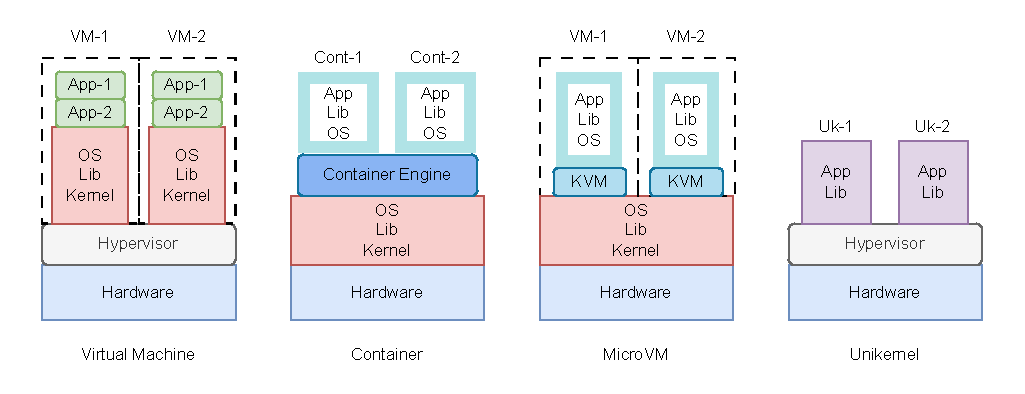
\includegraphics[width=0.75\textwidth]{resources/unikernel_overview.pdf}
    \caption{Different Virtualization Techniques}
\end{figure}

Unikernels \cite{madhavapeddy_unikernels_2013} provide an alternative to normal virtualization, as they are configured at compile time of the software that is to be executed on the virtual machine. The build system searches for dependencies of the software and only includes operating system parts that are actually used. This leads to a smaller attack vector as most software does not use all capabilities of a general-purpose operating system such as Linux, and it can potentially increase performance as unnecessary parts of the operating system are not executed as background processes. Unfortunately, this comes with the drawback of having a static image that needs to be recompiled when the software needs to be changed. In the following paragraph, we examine the unikernel framework Unikraft and its features that are crucial for our work. 

Unikraft \cite{Kuenzer_2021} is a unikernel known for its superior performance. Unikraft achieves this by having a flat and modular software hierarchy, grouping basic functionalities like memory management and networking into micro-libraries. These micro-libraries can then be configured at compile-time so that only necessary components are running alongside the main application. Furthermore, Unikraft aims to be POSIX- and Linux-compatible and executes binaries that are compiled for a Linux environment. To achieve this, Unikraft implements a shim layer for syscalls, which replaces actual system calls with library functions. No system calls also means that there is no kernel mode. Everything is done in the same address space, and there is no overhead for switching between user and kernel modes. This does decrease security; however, since unikernels are specifically compiled for one use case, there is only the main application that can cause damage to the system. Additionally, unikernels are intended to be run inside a virtual environment. In the case of an error, unikernels are rebooted quickly.

Unikraft supports networking via the lwIP library, which provides a TCP and an IP stack. lwIP was originally developed for embedded systems, but also has support for POSIX networking, which means it has a good tradeoff between compatibility and resource usage. Security mechanisms such as encryption and an SSL connection are done with OpenSSL, though currently Unikraft only supports major version 1.0.0 of OpenSSL, which is not sufficient for our purposes, as we will see later.
As a filesystem, Unikraft currently supports ramdisks as a static filesystem and external filesystems via the 9p filesystem protocol, which allows us to include external folders of the host system into the unikernel.

We decided on Unikraft because of its superior performance, our previous experience with it, and its very active community. Alternatives are the Hermit operating system and OSv.

%%
\chapter{Experiment}

Now we have seen the necessity for PQC, and we have seen the advantages that unikernels promise. With that, we now want to evaluate how PQC performs inside a unikernel on an embedded device. To do this, we developed a framework that can benchmark the primitive operations (keygen/encapsulation/decapsulation) of PQC algorithms as well as their performance inside a TLS benchmark. We also included containerization and native execution in the benchmark to compare the performance of post-quantum algorithms with different virtualization mechanisms.

\section{Setup}
The project consists of an OpenSSL application and a post-quantum primitives benchmark for all virtualization types. To build the project, the only requirements are a Unix environment and Docker. The global setup script in the top-level folder of the repository will build the project for Unikraft, Docker, and a native variant and create links in the respective folders (Unikraft, Docker, Native) to the OpenSSL application and the benchmark application. If you are on x86\_64, you need to enable multi-platform containers because the setup script requires the entire setup to be built on arm64. The exact commands are listed in the Appendix. 

To install the project, the system needs to be on the proper target system. The whole setup was developed on a Raspberry Pi 4B, but should be compatible with other arm64 machines, as long as they have a similar software setup. For software dependencies, it is expected to have QEMU and Docker installed. Suppose the project was not built on the target system. The \textit{send-to-pi.py} script in the repository can be used to sync all the changes to the target system, install the Docker container, and install the native OpenSSL library. Keep in mind that the script uses fixed paths, which may need to be changed. 

To run the project, the script generates a link to an OpenSSL application for each virtualization mechanism, e.g., \textit{Unikraft/openssl} runs OpenSSL inside a unikernel. This OpenSSL application closely resembles the regular cli application for OpenSSL, which can control most of the OpenSSL library, e.g., generating certificates or acting as an HTTPS server. However, the unikernel's version is custom and is limited to the \textit{s\_server}, \textit{s\_client}, and \textit{s\_speed} tools. We use these tools to check if we can establish a connection and to test the speed of connection establishment. The script also generates a link to a benchmark application that tests the speed of primitive operations of post-quantum algorithms, and it creates a test application (only for Unikraft) that runs post-quantum algorithms and checks the correctness of the output. Again, usage Examples are listed in the Appendix.

\section{Measurements}

The project contains several scripts inside the Benchmark directory. The \textit{run\_benchmarks.py} script executes all benchmarks when run without arguments. To limit the benchmarks to specific parameters (speed, memory, power) or only test specific algorithms, arguments can be specified that are also documented in the script. For a speed comparison, the script uses both OpenSSL and the benchmark application of the respective virtualization mechanism. To check the speed of primitive operations, it runs the benchmark application for a fixed amount of time (by default, 5 seconds), registers the number of operations that were done in that time, and calculates the mean of one execution. Similarly to this, it checks the speed of TLS connection establishment by creating connections for a fixed time (default 30 seconds) and also calculating the mean. For memory consumption, both applications are executed for a fixed time, and a memory profiler (top) creates regular samples of the memory usage. The results are saved in \textit{Benchmark/results/} in JSON format. 

Finally, power measurement is not done completely by the script but rather requires a manual setup. The script itself only runs the primitives or TLS connections and waits between different algorithms. Power needs to be measured with external hardware; we used the FNIRSI® FNB58 USB Fast Charge Tester. It needs to be connected to the target device and external computer that records the measured values, as displayed in Figure \ref{idp_setup}. The recording software is contained in the \textit{Benchmark/fnirsi\_usb\_power\_data\_logger} directory. It outputs a list of measured values (Voltage, Power, Energy) and the associated timestamps. The \textit{analyze\_power.py} script uses this output and calculates the power consumption for each specific algorithm, and also outputs it as a JSON file. Results are discussed in Chapter \ref{chapter:evaluation}. 


%% 
\chapter{Implementation}

In the previous chapters, we presented a high-level overview of how to use the project and how to execute benchmarks. Now we provide a more in-depth overview of the entire project. We will examine the structure of the repository and explain how the project is built. We show suitable technologies and why we chose them. We explain how they interact and what changes we made.

\section{Overview}

We started out with a native solution for our project that does not use any virtualization. The native solution is contained in the \textit{Native} directory, and it uses OpenSSL, as it is the most common library for TLS support. OpenSSL already provides a command-line interface, the openssl application, to create a basic HTTPS server and client for testing. For PQC algorithms, we use the liboqs library. We chose liboqs because it currently has support for the most post-quantum algorithms, and it also supports algorithms that are not standardized, in contrast to an official release of OpenSSL, which currently only supports ML-KEM, ML-DSA, and SLH-DSA. With OpenSSL's provider architecture, we can connect liboqs to OpenSSL, and can then access other algorithms such as FrodoKEM and HQC. Alternatives are regular OpenSSL and WolfSSL, which currently support ML-KEM, ML-DSA, and SLH-DSA, and more if we use custom versions. To test the performance of PQC primitive operations, we adapt the benchmarks from liboqs contained in the \textit{Native/oqs\_speed} directory for our benchmark application. When executing the setup script of the native directory, it will build all libraries from source and provide links to the OpenSSL application and the benchmark application inside the directory.

We then continued with the containerized solution. It has the same structure as the native solution, with the difference that it is built and run inside a Docker container with an Alpine Linux image. We picked Docker over other container solutions because of the widespread usage and support, and we picked Alpine Linux as it is widespread and because our laboratory already provided configuration scripts that work similarly to our native solution. The configuration is contained in the Container directory, and the setup script will create the container, again build the libraries from source, and create links to the benchmark and OpenSSL applications. It is important to consider that unless we have Alpine Linux installed on our target system, the standard library would probably be glibc instead of musl. For this reason, when the global setup script is used, the native solution is also statically built inside the container and then exported. This way, we get more comparable results later during the benchmark. 

\begin{figure}[h]
    \centering
	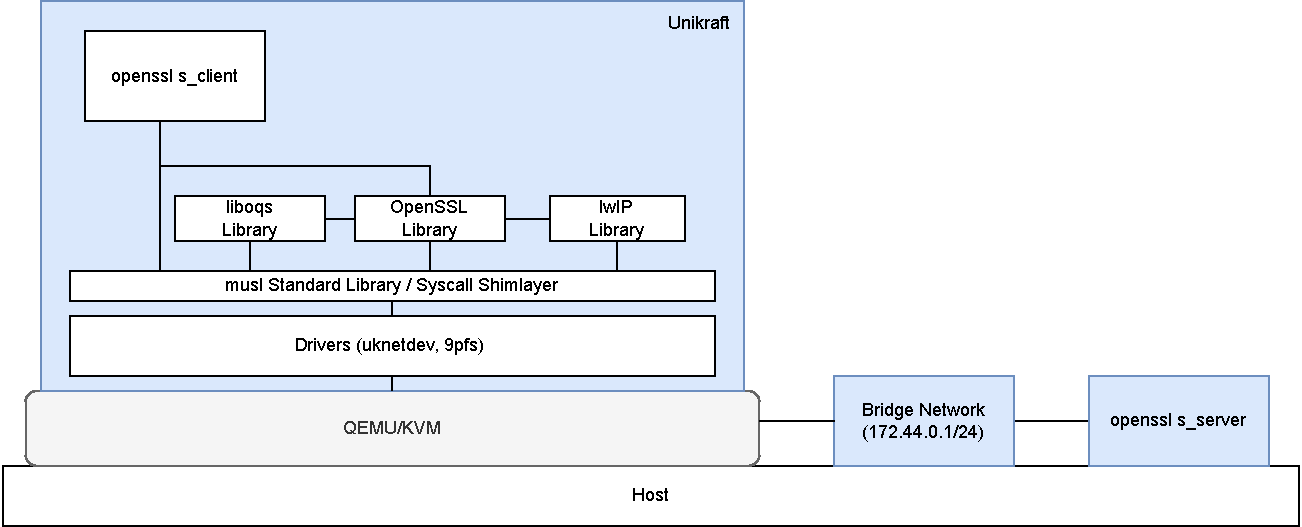
\includegraphics[width=0.8\textwidth]{resources/system_overview.pdf}
    \caption{Overview of all components of the system.}
    \label{idp_setup}
\end{figure}

Finally, we realized the unikernel solution. For a unikernel-based solution, we decided to use Unikraft, as discussed in Chapter \ref{chapter:background}. The unikernel solution is contained in the \textit{Unikraft} directory, and the setup script builds the libraries and the unikernel. The actual unikernel sources are contained in \textit{Unikraft/unikraft}. Since we compile our solution directly into the unikernel, we cannot reuse the same architecture as the native solution. Instead, we statically compile all needed libraries (OpenSSL, liboqs) and provide them to Unikraft as custom libraries inside the \textit{Unikraft/libs} folder. For the applications, we create several unikernels with different configurations. The first unikernel is contained in \textit{Unikraft/oqs\_uk\_speed} and runs the benchmark application on boot. The second unikernel is contained in \textit{Unikraft/ssl\_uk\_bin} and runs an adapted version of the OpenSSL application. The final unikernel is contained in \textit{Unikraft/ssl\_uk\_test}, and it runs liboqs's test suite. Again, the setup script creates links to the respective application, though instead of symbolic links, it creates scripts that launch a unikernel with a specific QEMU configuration. The following sections document the development process of the unikernel solution. It highlights the challenges we faced and our proposed solutions. 

\section{Integrating the Libraries in Unikraft}

Unikraft already has an older version of OpenSSL included in its core packages. Unfortunately, the version is too old to support the provider architecture for newer OpenSSL versions. So our approach was to integrate a newer OpenSSL version into Unikraft. 

Unikraft has its own build system, and the consensus in the Unikraft community is to create a new build script for each library that works on the original source files. This works well for smaller projects; however, with OpenSSL, we have several build steps we have to make before we get our resulting library, and all that is done with a large number of source files. 

To build OpenSSL, we first have to configure it via a Perl Configure script. This does contain the configuration for the main library, but also the configuration for a large number of tests, demos, documentation, and applications. This Configure script then generates a Makefile. Initially, we tried to include OpenSSL by rewriting the Makefile to work with the Unikraft build system, though this quickly turned out to be quite difficult, because of the size of the Makefile and the fact that most of it is generated automatically. This would also mean that if we tried to update the library, we potentially would have to rewrite the solution again. A proper solution for this problem would be to create a new target system in the Configuration script. However, we pursued another approach. Fortunately, the Unikraft build system also has the ability to include prebuilt object files and static libraries. We built a static library with OpenSSL and then used this feature to include it in Unikraft's build process. 

Another approach would have been to use the Unikraft elfloader project, which loads statically compiled binaries during runtime. We did not opt for this solution because regular Unikraft supports OpenSSL by compiling it directly into the unikernel. We wanted to make our solution as similar to the already existing infrastructure, in case the solution finds further usage in other projects.

Unikraft uses musl as a standard library, so we had to adjust our build process for the static libraries we wanted to include. We used musl-gcc to compile the library statically and then included it in the build script of our unikernel. We also needed to compile the Linux headers with musl-gcc because if they are compiled with regular gcc (with glibc), we have a different interface that is not compatible with Unikraft's interface. Aside from a few changes to fix mostly missing symbols and missing methods from Unikraft's musl implementation, we did not have to change much on Unikraft's side to successfully compile a unikernel. Since liboqs is fairly small and requires very little interfacing with the operating system, it loaded successfully with no change inside the unikernel. OpenSSL, on the other hand, did not run without any changes. 

OpenSSL has several constructors that are executed once the libraries are loaded (in our case, once the program is launched, since we have a static library). In one of those constructors, OpenSSL purposefully causes a false instruction to raise a SIGILL (signals illegal instruction) exception to detect CPU features. For a regular operating system, this does not pose a problem since CPU exceptions are caught by the kernel. In unikernels, though, the exception is not caught, and the unikernel simply crashes. We use a patch that forces OpenSSL to detect CPU features by using the auxiliary vector.

The current setup in the repository builds the libraries in the uk-build-aarch64 Dockerfile. Precompiled versions are already contained in the lib-openssl and lib-oqs libraries (only for arm64). 

\section{Using liboqs and Testing Primitives}

As mentioned before, the current version of OpenSSL has the ability to connect to a provider to use different cryptographic primitives. The liboqs project also has an oqs-provider component that connects to OpenSSL to let it use its primitives. Providers are typically contained in a separate file and are dynamically loaded by OpenSSL. This is currently not possible in our case because Unikraft has no support for dynamic loading. Fortunately, liboqs allows linking the oqs-provider statically and adds the oqs-provider to OpenSSL as a built-in provider. This way we can make use of liboqs components by recompiling our target application with a few added lines of code.

To make sure the included libraries are working properly, we extended the Unikraft test framework to include the OpenSSL and liboqs test suites. We used the tests that were already provided by the OQS project, both for the OQS library and the oqs-provider, limiting ourselves to the primitive operations that we later use for evaluation. Initially, the tests did not succeed and kept running infinitely. After stepping through the code of the compiled unikernel, we discovered that liboqs kept getting stuck on a recursive function. This function is used for liboqs's bignum implementation, and it was very likely that it caused a stack overflow. Fortunately, Unikraft's stack size is configurable, and after increasing the stack size to 8 pages, all tests ran successfully. 

To test the speed of primitive operations, we compiled the liboqs's test suite into a unikernel. This also required little change since, apart from the build system, Unikraft is aiming to be compatible with a Linux environment. 

\section{Setting up the OpenSSL Application}

Now that we have the benchmark application running inside a unikernel, we also wanted to run the OpenSSL application. 
To do this, we first had to compile the OpenSSL application source in the unikernel. The OpenSSL application is built modularly and allows partial compilation to only include a subset of the available commands. We opted for only including the \textit{s\_server}, \textit{s\_client}, and \textit{s\_speed} sources because these were sufficient for testing a connection and benchmarking. We included the sources, created and configured the build system for the unikernel. The initial build was running, though it was not possible to make a connection yet. The reason for this is that Unikraft requires manual configuration of the network. 

\begin{figure}[h]
    \centering
	\includegraphics[width=0.5\textwidth]{resources/idp_setup.pdf}
    \caption{Setup of the Power Measurement Benchmark.}
    \label{idp_setup}
\end{figure}

To enable networking in Unikraft, we need to include the Unikraft port of the lwIP library, which includes a TCP and IP stack. We also need to enable the uknetdev driver (and LIBUKNETDEV\_EINFO\_LIBPARAM) to have a networking device that we can send data on. Now we can perform network operations inside the unikernel, though they do not reach our host network yet. Since we boot the unikernel with QEMU as a hypervisor, we have to configure QEMU to connect to our host network. There are several ways to configure networking\footnote{\url{https://wiki.qemu.org/Documentation/Networking}}, though the Unikraft community recommends the use of a bridge network because of its superior performance. We create a network bridge on our host system and assign it an IP address. Then we configure QEMU to use said bridge, and we pass the IP address to the unikernel. Now, when the unikernel sends a message, QEMU automatically passes the network packages to the bridge, and we can communicate with the unikernel via the bridge. The bridge setup is already included in the setup commands in the Appendix. 

We can now make a TLS connection; however, we cannot check certificates yet. The openssl application can only check certificates from the filesystem. Compiling certificates into the unikernel and accessing them directly is certainly possible; however, this would need major changes in the OpenSSL application code. Instead, we opted to enable full filesystem support inside the unikernel. Since we only load files in the beginning and not during a benchmark, the impact is negligible. Similar to Docker's bind mount, where folders of the host system can be mounted inside a container, Unikraft can achieve a similar result with the 9p filesystem protocol. 9p is a networking protocol that can remotely connect to a filesystem. It is already built into Unikraft and only needs to be enabled in the configuration. We can set a path in the QEMU launch parameters and pass the filesystem to the unikernel (Note: 9pfs does link the mounted folder as the root directory, which means we cannot use absolute paths for certificate files). Now we can verify certificates that were signed with post-quantum digital signatures. 

To use post-quantum key exchange algorithms, we still need to make some changes. The TLS protocol lets a client choose a list of key exchange groups that it supports before making the server choose between those solutions. By only issuing one allowed group as the server, we can force the client to use this specific group. To make sure the client accepts, we also need to configure the supported groups. We can do so by changing the OpenSSL config file. Fortunately, we now have filesystem support, which means we can load a custom config file. To add the post-quantum groups, we need to add them to the DEFAULT\_GROUPS field in the config file (Note: the group names are inconsistent; look here\footnote{\url{https://github.com/open-quantum-safe/oqs-provider/blob/main/ALGORITHMS.md}} for proper names). Now we can also choose custom key exchange algorithms, including post-quantum KEM.

\section{Performance Optimizations}

During development, we examined how to reduce the unikernel's overhead. The first configuration we tried was compiling the unikernel with link-time optimization, though this did not seem to show any obvious improvements for the smaller tests we executed manually. Because of this and because link-time optimization is still experimental, we decided not to enable it in the benchmarks. The second configuration that we considered was hardware acceleration with kvm. We deem kvm an important optimization, as otherwise our hypervisor QEMU would fall back to code emulation via a tiny code generator, which has a vast overhead. kvm utilizes hardware extensions to run a virtual machine directly on the hardware and only switches to the hypervisor when specific instructions are executed or specific data sections are accessed. Unfortunately, enabling kvm caused the unikernel to crash with a major CPU exception. All libraries that implement cryptographic operations require a way to get random data, which is either done through the /dev/random device or the getrandom syscall on Linux. We configured the libraries inside Unikraft to use the getrandom syscall, which on arm64 used an assembly instruction to generate a random value. However, our target system (Raspberry Pi 4B) does not support these arm64 instructions to generate randomness and would instead generate an exception because of the missing instruction. Fortunately, Unikraft provides a way to accept a seed and use software-based randomness instead of hardware randomness. Currently, each time a unikernel is launched, a random value is generated by the host operating system and passed to the unikernel. The unikernel uses this value until it shuts down. However, this can negatively impact security if we have a particularly long-running unikernel. Since the scope of this work lies in performance, we do not pursue this security impact any further. 

\section{On the Usability of Unikraft}

During our work, we worked extensively with the Unikraft unikernel and made several impressions. First and foremost, Unikraft is in early development, the project is actively being worked on, and it has a very vibrant community, which means most problems will very likely be solved in the future, and for most problems, the community has solutions ready. With that said, Unikraft has flaws that need to be addressed: Unikraft's build system works similarly to the Linux kernel configuration. Each unikernel gets a kernel config (similar to kconfig) that a developer needs to configure manually before they can compile the project. Efficiently working with this system requires a developer to have previous knowledge, as all libraries and capabilities have to be managed manually, and often there are obscure rules for the configurations for the unikernel to function at all (e.g., for ARMv8, no specific architecture must be specified, LIBUKNETDEV\_EINFO\_LIBPARAM for networking, multiple TTYs which do not work in specific situations). As mentioned before, the projects are in extensive development; however, much of the code is provided by the community, which results in lots of unmaintained code, even for important projects, e.g., musl, to the point where community members actively provide fixes, but they are ignored by Unikraft's developers. 
Unikraft's build system is based on make and has not changed much since the initial proposal of the project, though currently building a Unikraft unikernel with an example application throws many warnings (e.g., because of missing syscall implementations). The build system was also originally designed for all libraries to be included in the unikernel itself. However, later the developers decided to move some libraries out of the unikernel (e.g., musl or lwip for networking) and provide them externally. As the build system was not developed for external libraries, changing only a single file resulted in the recompilation of the entire unikernel. On our system (consumer device), the build time was in the range of minutes, though this adds up when prototyping a solution. When creating a port for a library, it is expected that the port is created from the source of the library, which requires more effort, and since the Unikraft project heavily depends on the community, there is less motivation to create ports. A newer approach is instead to ignore the build system (and the libraries) and ship prebuilt unikernels that use ELF loading to load a Linux application. However, with this approach, we lose many possibilities for optimization because we have to compile the unikernel with everything. Furthermore, ELF loading only supports static linking, which means it has low compatibility with Linux binaries that almost always require glibc dynamic loading. Even if we compile an application statically with glibc, glibc is still dependent on dynamic loading for certain features. Unikraft also has no simultaneous multithreading, which means if we want to use multiple cores, we would need to launch multiple unikernels and communicate between them via the network. Finally, Unikraft does not have complete binary compatibility with Linux yet (e.g., standard libraries have missing functions). 

%% 
\chapter{Evaluation}
\label{chapter:evaluation}

In this chapter, we evaluate the performance of our implementation and compare it to a native implementation and a containerized version running on the same hardware. We will first give an overview of the performed benchmarks and their respective setup, and afterward examine the results. Generally, we differentiate between a primitive benchmark and a TLS benchmark. Primitives are split into three operations (with the exception of ECDHE, which only has two operations: Key Generation and Key Deduction): Key Generation, Encapsulation, and Decapsulation for the KEM primitives and Key Generation, Signing, and Verifying for Digital Signatures. We measure each operation separately. For TLS, we chose a subset of combinations of key exchange and signature algorithms and measured the connection speed. We first explain how we set up the benchmark, next we describe the measured results, and in further paragraphs we discuss the findings. Overhead refers to the increased execution time, amount of connections, memory consumption, or energy consumption (e.g. $\textnormal{OVERHEAD}(\textnormal{env}) = \frac{\textnormal{TIME}(\textnormal{env})}{\textnormal{TIME}(\textnormal{native})}$).

\section{Speed}

\begin{figure}[h]
    \centering
	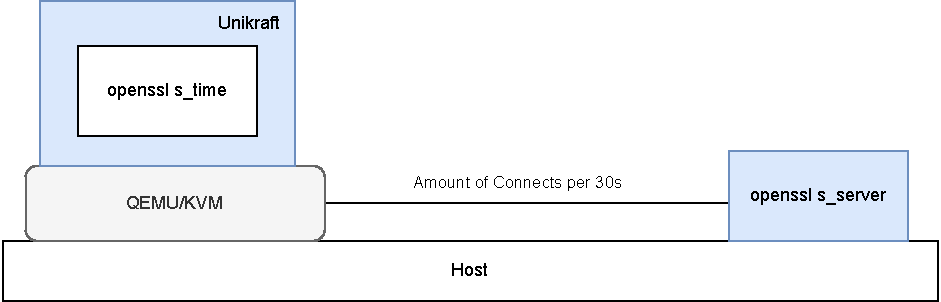
\includegraphics[width=0.7\textwidth]{resources/speed_overview.pdf}
    \caption{Overview of the speed benchmark setup.}
    \label{idp_setup}
\end{figure}

To test the speed of the primitive operations, we use the provided liboqs benchmarks and adapt them to run inside the container and the unikernel. We also add primitives from classical PKC that are implemented in OpenSSL, mainly ECDHE for key exchange and ECDSA, RSA for digital signatures. The benchmark runs for a fixed amount of time (5 seconds) and computes the number of operations the application was able to do in this timespan. We compute the result for all three operations of the primitives (with the Exception of ECDHE). The results are displayed in \ref{fig:table_primitives_speed}. We first compare results between different primitives, and then we compare the performance between different virtualization mechanisms. 

Kyber has the best performance of all post-quantum ciphers, even with larger keys. Kyber inside a container produces very similar results and only produces a slight overhead. Inside a unikernel, Kyber performs marginally worse, taking almost double the amount of time when compared to a native execution. BIKE is taking vastly more time than Kyber for all operations, about 400x times for encapsulation. Again, containerization performs very similarly. The unikernel has about 1.25x overhead. For HQC, we get a better performance for generation, though worse for encapsulation and decapsulation. Containerization is comparable to a native execution. On the unikernel, we get a slightly slower result with an overhead of 1.3x. FrodoKEM-SHAKE performs very similarly to HQC but has better performance for de- and encapsulation. Unikernel execution is slightly faster, though only a 1.5 percent speedup is measurable. For FrodoKEM-AES, the performance is much worse, about 3 times slower. On the unikernel, the performance is also slightly better than both container and native execution, with a speedup of 10 percent. Our litmus test ECDHE performs similarly to Kyber, and we see that all execution styles are the same.

\begin{figure}[h]
    \centering
	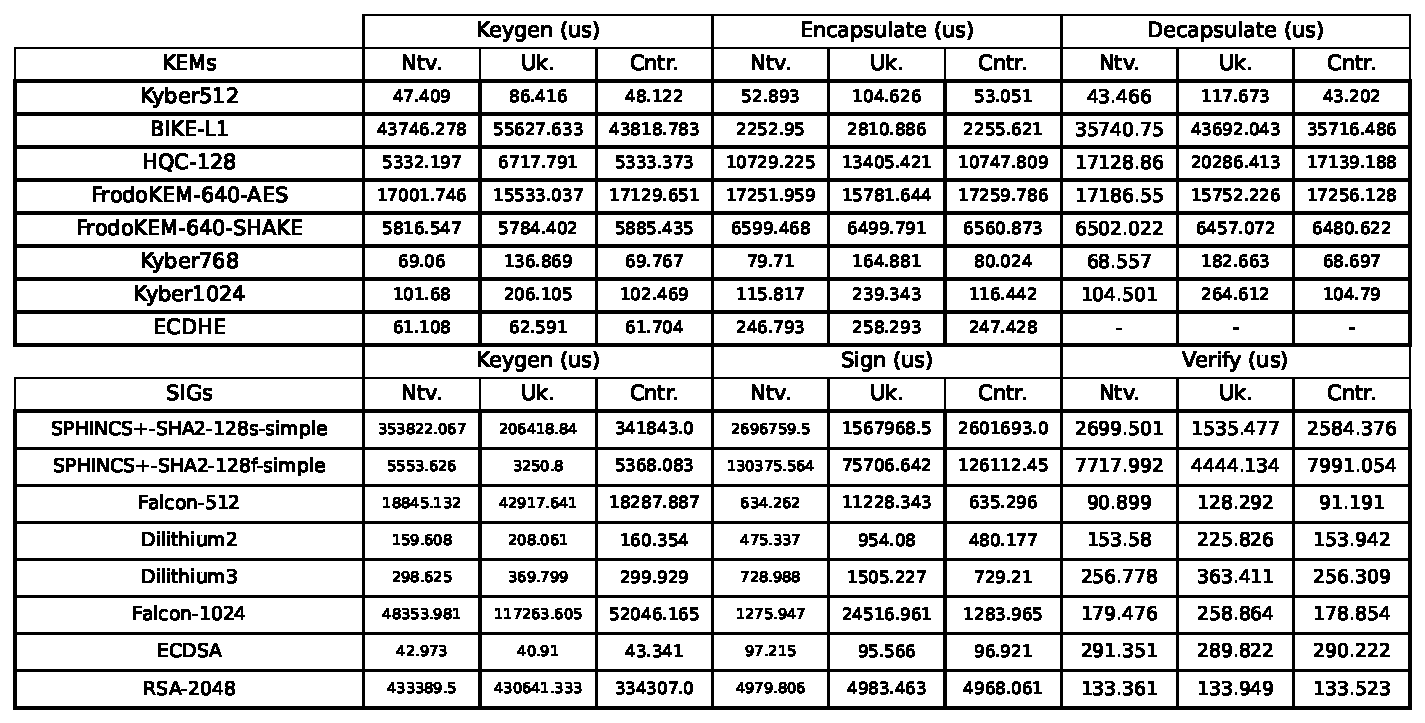
\includegraphics[width=1\textwidth]{resources/table_primitives_speed.pdf}
    \caption{Time (\mu s) of Traditional and Post-quantum Primitives.}
    \label{fig:table_primitives_speed}
\end{figure}

Now, going to the signature algorithms, we can see that the first algorithm, SPHINCS+ (the small variant), performs significantly worse for all operations when compared to ECDSA. On a Container, we get similar results to native execution, and on a unikernel, it performs marginally better with a speedup of 1.75. For the fast variant, we get much faster speeds on keygen and sign operations; however, on the verify operations, our results are slower. The overhead between different execution styles is similar to that of the small SPHINCS+ variant. The next signature algorithm, Falcon, performs significantly worse than ECDSA for key generation, but for sign operations, it only performs slightly worse, and the verify operation is faster. Container execution is similar, and inside a unikernel, we get an overhead of about 2.2x for key operations, 17.7x for signing, and 1.4x for signing. For bigger key sizes, the execution time doubles, but the relative overhead stays the same. Finally, we examine the Dilithium algorithm, which has arguably the best performance among post-quantum signature algorithms. For keygen and sign operations, it has an overhead of 4x compared to ECDSA, and its verify operation has a speedup of 2x. Again, Container execution time is similar, and unikernel execution takes roughly 1.3-2.0x more time. For larger key sizes, the execution time roughly doubles, and the relative overhead stays the same.

For all algorithms, the unikernels' results differ quite a lot when compared to native and container execution. We suspect there are two reasons for this result. The first reason is likely because of how unikernels are built. Although they are quite minimal, unikernels are still a complete operating system running inside of a hypervisor, which means during execution of an algorithm, we also have to factor in memory management, scheduling, and I/O operations. Furthermore, all of this is done on one core, as Unikraft currently has no proper support for simultaneous multithreading. The second reason is that we do not use hardware-generated entropy when using the unikernel; it only receives a seed upon booting, which is used for its entire lifespan. If there are algorithms that need randomness and they request it from the operating system, the operating system then uses hardware instructions or measures peripheral latency to get entropy. The unikernel only uses a pseudo-random number generator with the provided seed, which is much faster. This will create a larger overhead on the native and container versions and result in a faster execution time on unikernels for SPHINCS+ and FrodoKEM.

To test the speed of the TLS connections, we use the openssl \textit{s\_server} and \textit{s\_time} application and adapt them to run inside the container and the unikernel. First, we generate certificate chains with the selected digital signature algorithms, and afterward, we run \textit{s\_time} for a fixed amount of time (30 seconds) and compute the number of operations the application was able to do in this timespan. We only look at the connection establishment of a new connection and neglect connections with session reuse, though the results are still available in the raw data. The results are displayed in \ref{fig:bar_tls_speed}. We limit ourselves to a subset of combinations of different digital signature and key exchange algorithms; we take the same subset as \cite{tasopoulos2023energy} for a better comparison. We first compare the results between different primitives and then between different virtualization mechanisms.

\begin{figure}[h]
    \centering
	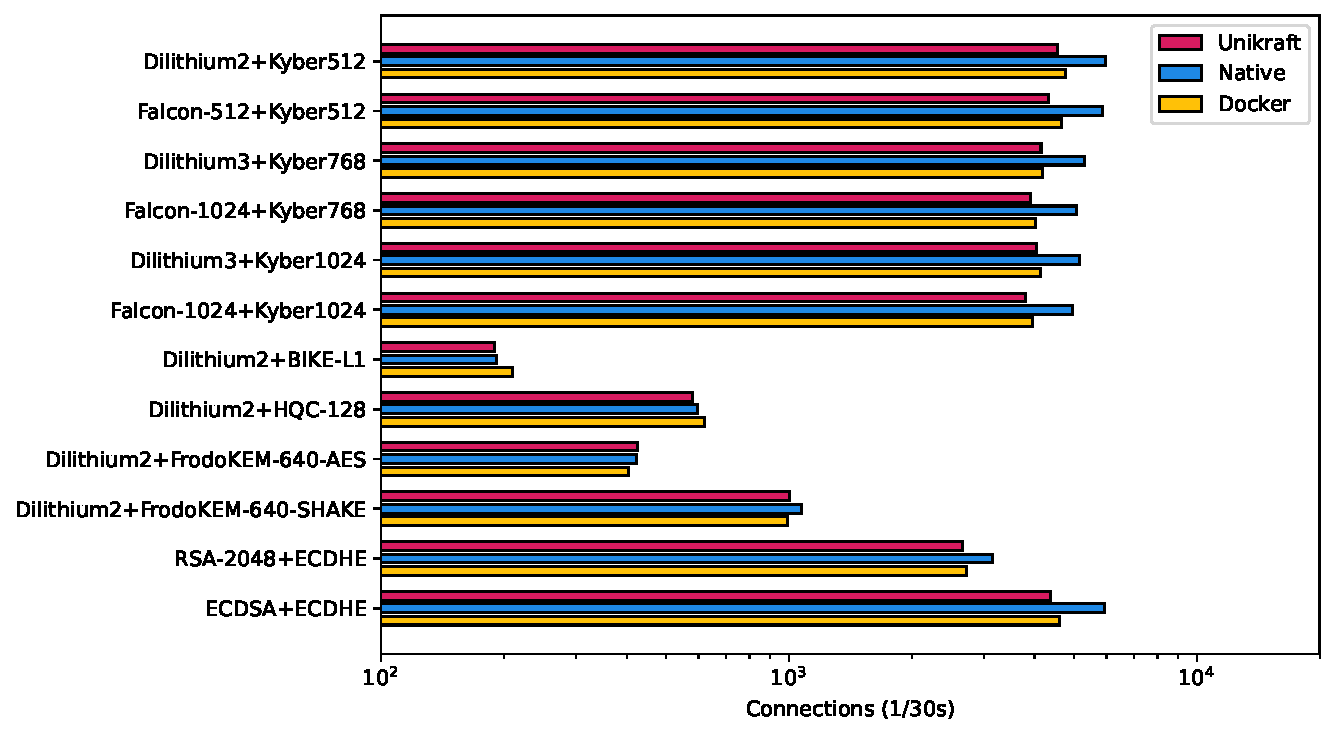
\includegraphics[width=1\textwidth]{resources/bar_tls_speed.pdf}
    \caption{TLS Connections of Traditional and PQ TLS 1.3 handshakes}
    \label{fig:bar_tls_speed}
\end{figure}

The first combination is Dilithium and Kyber, which have a very similar performance when compared with a regular TLS handshake with ECDSA and ECDHE. When comparing different virtualization mechanisms, we can now see that native execution has the expected advantage over virtualization. Docker and Unikraft are almost on par performance-wise, with Docker only having a slight advantage. Now, if we look at the results on different NIST levels of Dilithium and Kyber, we can see that the performance only barely decreases, but we get added security. The difference between virtualization mechanisms stays consistent. If we look at the combination of Falcon and Kyber, we can see that the results are slightly lower than with Dilithium and Kyber, and their performance characteristics stay the same on different NIST levels and different virtualization mechanisms. Taking a look at the combination Dilithium and BIKE, we can see that we have a low amount of connections with an overhead of roughly 27.6x. Here, Docker performs minimally better, and the native execution and unikernel execution are on par. For Dilithium and HQC, we get a better result, but still a low performance with an overhead of 9.1x. Between virtualization mechanisms, they perform similarly to Dilithium and BIKE. If we look at Dilithium and FrodoKEM, we get different results depending on the symmetric encryption algorithm that FrodoKEM uses. If we use AES, we get an overhead of 13.2x, and if we use SHAKE, we get an overhead of 5.3x. Again, the performance of all virtualization mechanisms is very similar; for the AES variant, the unikernel has a slightly higher result, and Docker has the lowest. For SHAKE, the native execution has the highest amount of connections, and Docker and Unikraft are on par.

Most of the overhead of the ciphers between different virtualization mechanisms is negligible. We suspect that it is because we only execute the PQC algorithms once per connection, and for each connection, the network stack creates an additional overhead that is now also visible in the benchmark. For the combinations that contain BIKE and HQC, Docker outperforms other execution styles. We suspect this is because we use a Docker image based on Alpine Linux. Alpine Linux uses musl as a standard library instead of glibc, which can have a positive impact on performance in certain scenarios, as musl is kept very minimal and thus has better cache behavior for small applications.

\section{Memory}

\begin{figure}[h]
    \centering
	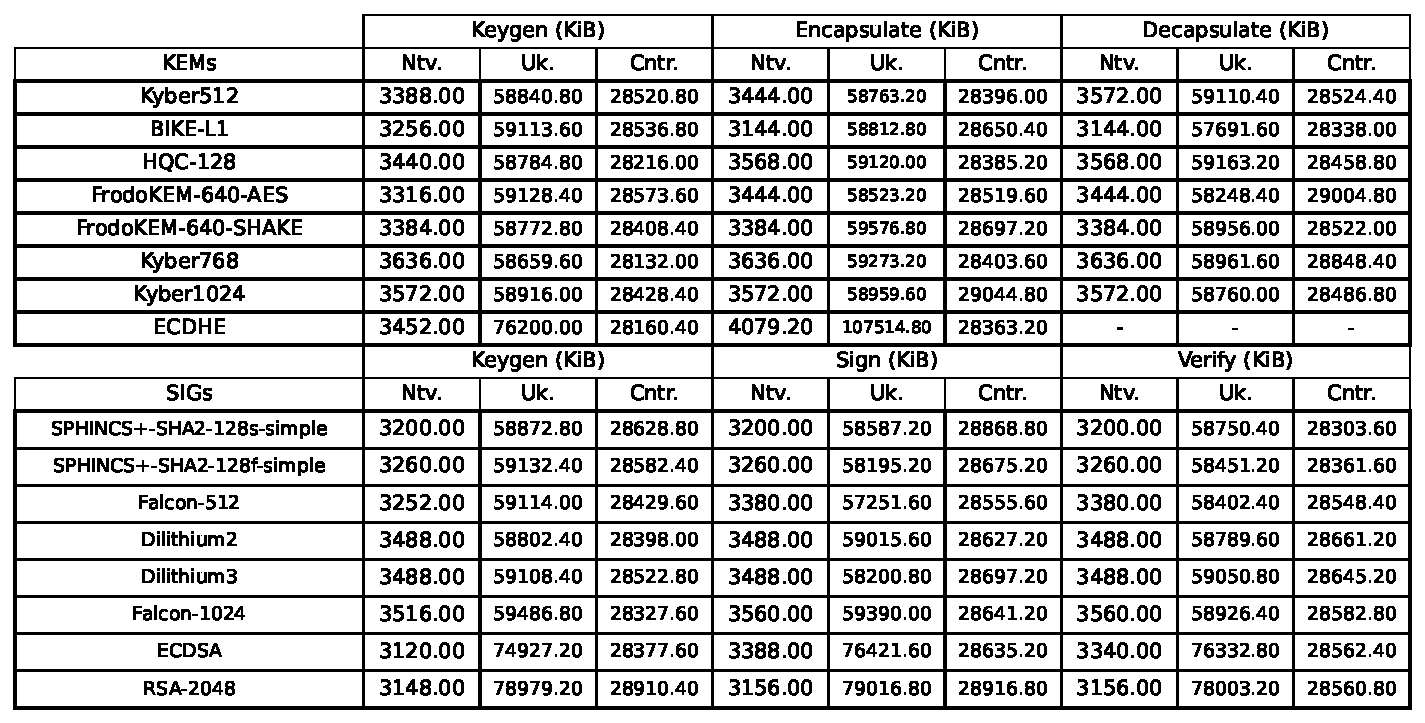
\includegraphics[width=1\textwidth]{resources/table_primitives_memory.pdf}
    \caption{Memory (KiB) of Traditional and Post-quantum Primitives.}
\end{figure}

To test the memory consumption of all virtualization mechanisms, we ran the regular benchmark again for both primitive operations and TLS connections, and during execution, we took regular usage samples of the program with a memory profiler\footnote{https://www.man7.org/linux/man-pages/man1/top.1.html} for a fixed amount of time (5 seconds for primitive execution, 30 seconds for TLS connections). We then calculated the average amount of memory that was used during execution. We only considered the actual physical memory that was used and reported by top. Usage of virtual memory is also available in the raw results. Again, we first examine the results of only the primitive execution and then consider TLS connections.

If we look at the native execution of the algorithms, we can see that different algorithms use between 3.2 and 3.7 MB. The same is happening when using a container, where we get between 28 and 30 MB of memory usage. The unikernel also uses a consistent amount of memory between 58 and 60 MB; however, when running classical key exchange or digital signature algorithms, we get a higher memory usage between 76 and 80 MB. 

The impact of different algorithms is minimal, and the fluctuations in the results mostly stem from the operating system,  because of different allocation strategies or entropy generation. We can confirm this by looking at different NIST levels of the same algorithm, which show less memory usage for higher NIST levels. This applies to the native and containerized solutions. The unikraft solution uses considerably more memory when working with non-post-quantum algorithms. For non-post-quantum algorithms, we use the OpenSSL library (instead of liboqs), which has a higher complexity when setting up a key exchange or digital signature, including the allocation of many OpenSSL-specific objects. We suspect that Unikraft's and or QEMU's allocators are not able to handle this as efficiently as the native and containerized solutions. 

For TLS connections, the results are similar. For native execution, we get between 12 and 14 MB, for container execution, between 28 and 30 MB, and for unikernel execution, we get between 110 and 120 MB of memory usage. The exact results are listed in the Appendix.

\section{Energy}

\begin{figure}[h]
    \centering
	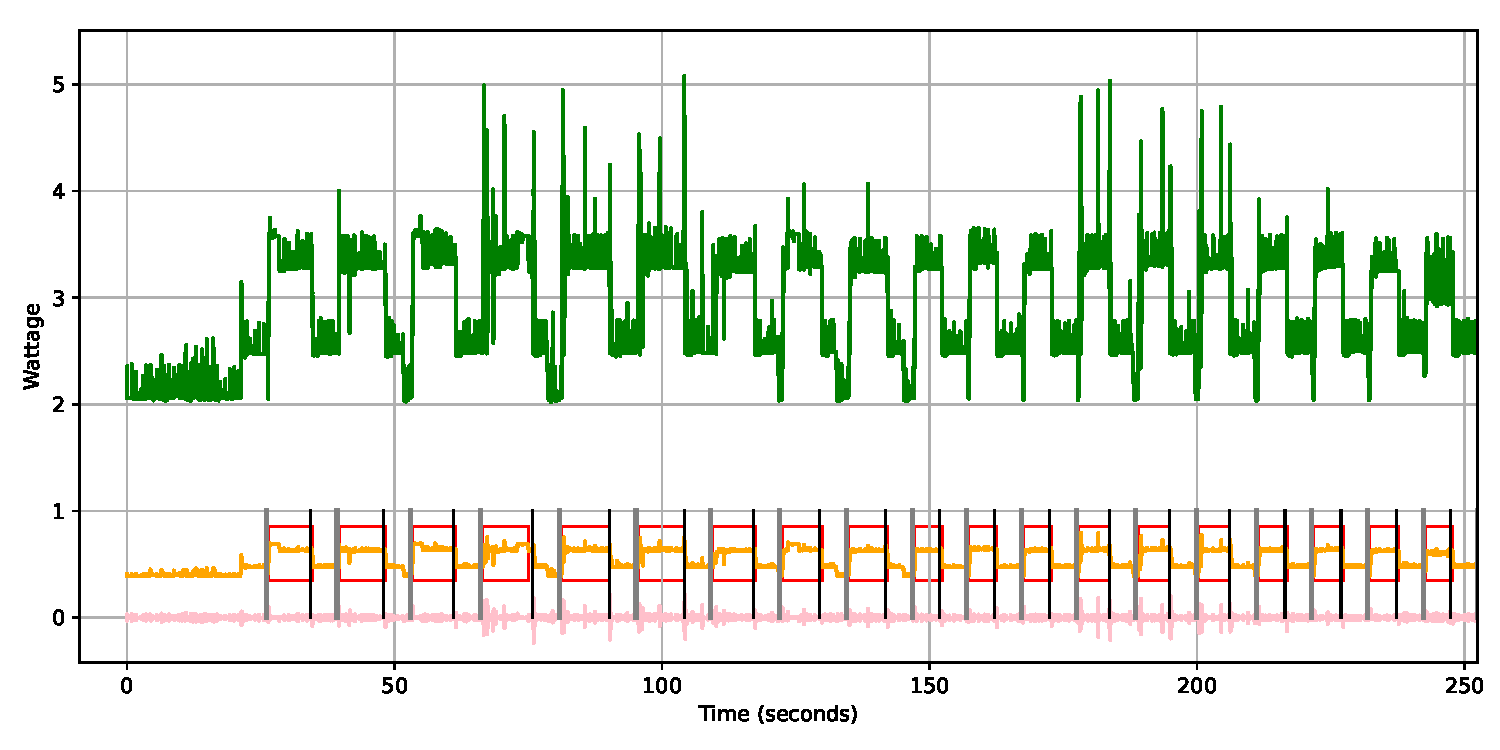
\includegraphics[width=1\textwidth]{resources/analyze_wattage.pdf}
    \caption{Analyzing the Output of the Fnirsi Recording Script.}
    \label{fig:analyze_wattage}
\end{figure}

In our setup, measuring energy consumption is not automatic, and we need to perform several steps in order to get the results.
We perform energy measurement with an external hardware, the FNIRSI® FNB58 USB Fast Charge Tester, which we connect to our target system and an additional computer to record the energy consumption of the target system. We manually start recording on our second computer, and then we start our benchmark. The benchmark executes all primitive operations and TLS connections for a fixed amount of time (5 seconds for each primitive operation and 30 seconds for TLS connections, a combination of algorithms). After the benchmark is finished, we now have all the results as a list of measured values (Voltage, Power, Energy) and associated timestamps. 

Now we need to find out which values belong to the timespan during which a specific algorithm was executed. We did this by bringing the results into a visual format and then finding a way to reliably predict the start and the end of each algorithm. We can see in Figure \ref{fig:analyze_wattage} the power in green and the current in yellow. On our target system, the electric potential was around 5V with minor fluctuations. The goal is to detect when an algorithm is starting and when it stops. We decided to use the delta of the current to register a started algorithm when the change is large enough. We chose the current because it has fewer fluctuations compared to the power, and we applied a batch average of 3 to account for the remaining fluctuations in the current. During the execution of the benchmark, we also saved the start and stop times of each algorithm (marked in grey) so that we can narrow down our search for the proper starting time. With this approach, we were able to measure the power and energy consumption of each algorithm individually and together with a TLS connection. We measure the energy consumption of each algorithm over a fixed time. We do not consider energy consumption that is needed to execute a specific algorithm once, because if we did, our results would look very similar to the speed benchmark. When we consider the energy consumption over a fixed time, we can test the actual behavior of an algorithm more accurately. 

\begin{figure}[h]
    \centering
	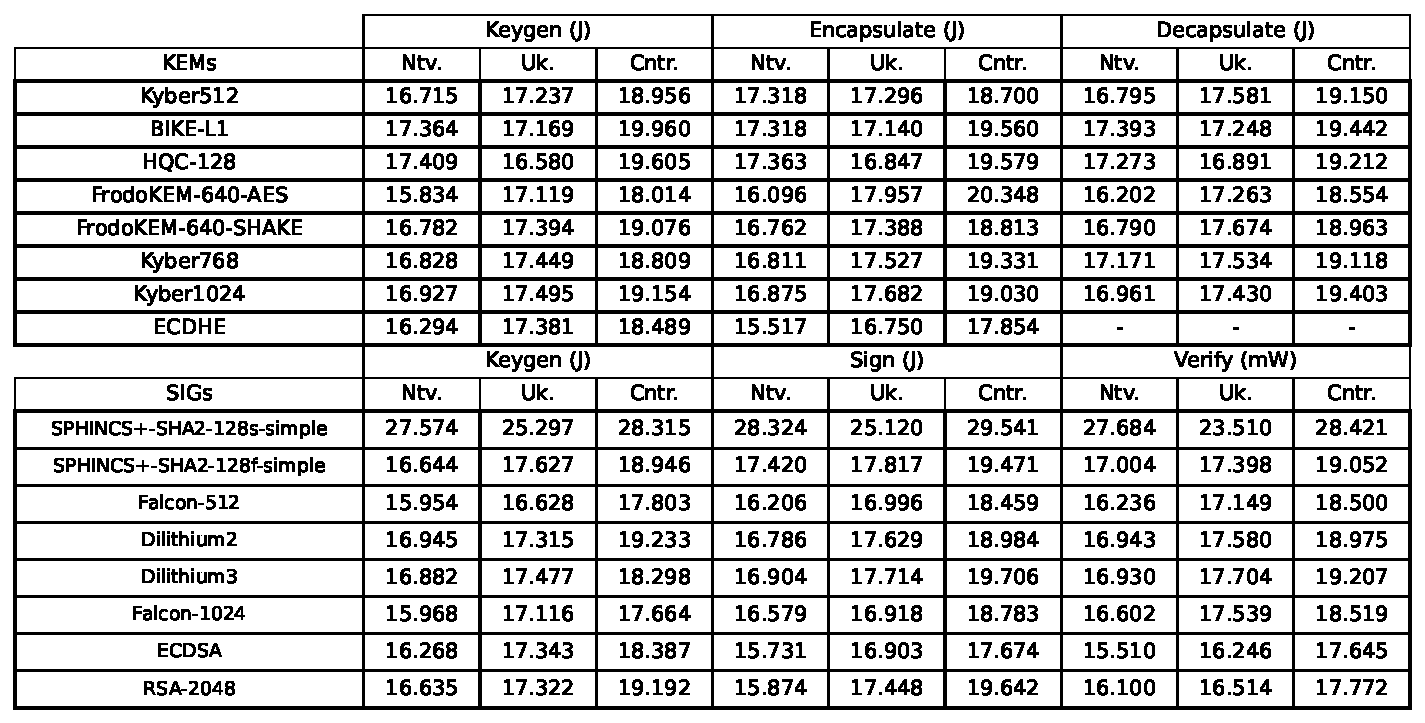
\includegraphics[width=1\textwidth]{resources/table_primitives_energy.pdf}
    \caption{Energy Consumption (J) of Traditional and Post-quantum Primitives.}
    \label{fig:table_primitives_energy}
\end{figure}

If we look at the results of key exchange algorithms in Figure \ref{fig:table_primitives_energy}, we can see that the energy consumption of all primitives is generally really similar. Energy consumption is in the range of 16 to 18J for the native execution for all operations. ECDHE has the lowest power consumption with 16.3J/15.5J, and the highest power consumption was reported by BIKE and HQC with 17.3J for all operations. If we compare different virtualization mechanisms, we can see that, on average, the unikernel performs very similarly to and sometimes even outperforms the native execution (in the case of HQC). Containerization has a slight overhead with, on average, 1-2 additional Jouls when compared to native execution. If we look at digital signature algorithms, the results are very similar to the key exchange algorithms. We also have about the same amount of energy consumption for each algorithm, except for SPHINCS+. In addition, we have the same overhead when comparing different virtualization mechanisms. SPHINCS+s, on the other hand, has a big overhead jumping to 27-23 additional Joules for all virtualization mechanisms. Container execution again has a slight overhead for SPHINCS+s, while unikernel execution requires less energy than the native execution.

For the high energy consumption of SPHINCS+s, we suspect that this is because the s-variant of SPHINCS+ was designed for space optimality, so that during the algorithm, only a small amount of memory is used, which means we get higher IPC and can thus also consume more energy. Furthermore, as mentioned in the speed comparison, SPHINCS+ requires more entropy than other algorithms. Entropy, which we only have to gather on native execution and inside the container, since the unikernel does not have the capability to generate randomness itself, but relies on the host system. We suspect that because of this, we gather less entropy for the unikernel and thus also require less energy. We also collected the power consumption of the target system, though, because the results were very similar to the previous results, we will not discuss them further. They are listed in the Appendix.

\begin{figure}[h]
    \centering
	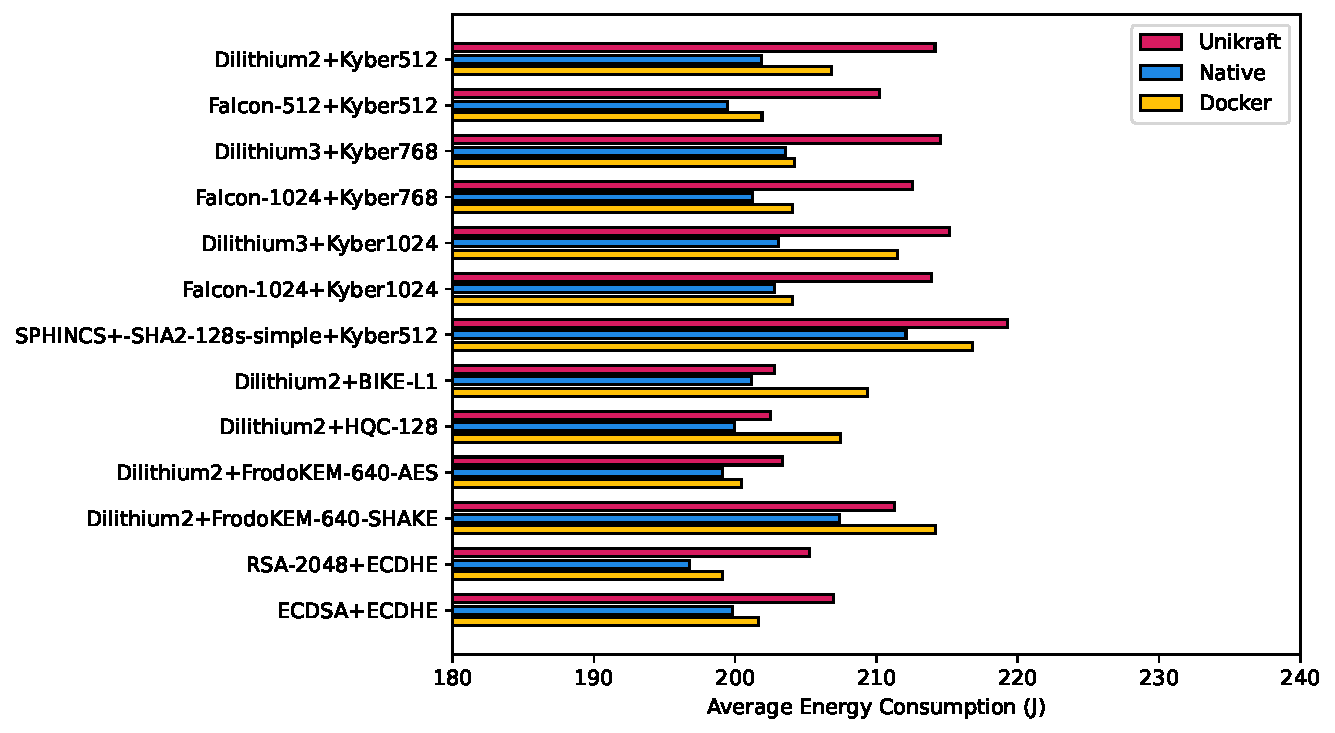
\includegraphics[width=1\textwidth]{resources/bar_tls_energy.pdf}
    \caption{Energy Consumption of Traditional and PQ TLS 1.3 handshakes}
    \label{fig:bar_tls_energy}
\end{figure}


Finally, we look at the energy consumption of TLS connections. We also measure the consumption over a fixed timespan and do not measure energy consumption per connection. We can see in Figure \ref{fig:bar_tls_energy} that again, when comparing different combinations of algorithms, the results are very similar. However, when comparing different virtualization mechanisms, we get a more noticeable result. Unikernel execution can have an overhead of up to 10J in the case of Dilithium and Kyber. For algorithms that were considered faster, we generally get a higher overhead when using unikernel execution compared to container execution (e.g., with Dilithium, Falcon, and Kyber). For slower algorithms, container execution has a higher overhead than unikernel execution (e.g., with BIKE, HQC, FrodoKEM). The most efficient algorithm in terms of energy consumption is FrodoKEM-AES, and the most inefficient is SPHINCS+s. Again, we also tested power consumption, though the results are similar to energy consumption, which is why they are not discussed and can be found in the Appendix.




%% 
\chapter{Conclusion}

In this work, we implemented a framework to test post-quantum algorithms with different virtualization mechanisms in terms of speed, memory usage, and energy consumption. Our primary focus was on the performance of the unikernel. We discovered that for the raw execution of the post-quantum algorithms, the results for virtualization mechanisms actually differ. However, when considering them inside a TLS connection, their primary use, the difference becomes less noticeable to the point where it does not matter to differentiate between different virtualization mechanisms. In terms of speed, the unikernel is slightly slower than a container execution when averaging the test results. Memory usage is generally higher, and power consumption is roughly the same as container execution. Additionally, since unikernels have a much higher overhead for development and maintenance, we do not recommend the general usage of a unikernel in resource-constrained environments with post-quantum cryptography. If we have a scenario where we need fast boot times of a virtual machine (e.g., AWS Lambda), then a unikernel does make sense.


%%
\printbibliography

%%
\chapter{Appendix}


\section{Setup Commands}

For the setup, create a virtual bridge network and then run the setup script:

\begin{lstlisting}[style=shell]

sudo ip link add dev virbr0 type bridge
sudo ip address add 172.44.0.1/24 dev virbr0
sudo ip link set dev virbr0 up

sudo mkdir /etc/qemu
sudo echo "allow virbr0" > /etc/qemu/bridge.conf

./setup.sh

\end{lstlisting}

Note: If you are on x86\_64/amd64, you need multi-platform support as the setup script requires the entire setup to be built on arm64/aarch64. Run the command below to enable multi-platform support:

\begin{lstlisting}[style=shell]
docker run --privileged --rm tonistiigi/binfmt --install all
\end{lstlisting}


\section{Usage Examples}

The setup script will generate a link to an OpenSSL binary with the correct virtualization, e.g., Unikraft/openssl runs OpenSSL inside a unikernel. Before we can execute openssl \textit{s\_server}/\textit{s\_time} commands, we need a public key infrastructure. The commands to establish such an infrastructure are also listed below. 

\begin{lstlisting}[style=shell]
Native/openssl req -x509 -new \
			-newkey dilithium3 \
			-keyout pki/CA_dil.key -out pki/CA_dil.crt \
			-nodes -subj "/CN=Test CA" -days 365

Native/openssl req -new \
			-newkey dilithium3 \
			-keyout pki/server_dil.key -out pki/server_dil.csr \
			-nodes -subj "/CN=testserver"

Native/openssl x509 -req \
			-in pki/server_dil.csr -out pki/server_dil.crt \
			-CA pki/CA_dil.crt -CAkey pki/CA_dil.key -CAcreateserial -days 365
\end{lstlisting}

Below are examples of how the \textit{s\_server}/\textit{s\_time} applications are used to measure the TLS connections.
Note: Unikernels are reachable via 172.44.0.1/24 and Containers via the host. docker.internal

\begin{lstlisting}[style=shell]

Native/openssl s_server  -key pki/server_dil.key -cert pki/server_dil.crt \
                         -accept 443 -www
Unikraft/openssl s_time  -connect 172.44.0.1:443 -CAfile pki/CA_dil.crt -www /

Native/openssl s_server  -key pki/server_dil.key -cert pki/server_dil.crt \
                         -accept 443 -www
Container/openssl s_time -connect host. Docker.internal:443 \
                         -CAfile pki/CA_dil.crt -www / 

Native/openssl s_server  -key pki/server_dil.key -cert pki/server_dil.crt \
                         -accept 443 -www
Native/openssl s_time    -connect localhost:443 -www / -CAfile pki/CA_dil.crt
\end{lstlisting}
To measure the primitive operation's speed, the setup script provides benchmark scripts that measure keygen/sign/verify and keygen/encapsulate/decapsulate operations of the OQS library:

\begin{lstlisting}[style=shell]
Unikraft/benchmark sig --no_keygen --no_sign ECDSA
Native/benchmark kem -d 5 --no_keygen ECDHE
Container/benchmark kem --no_keygen --no_encaps Kyber512
\end{lstlisting}

To execute tests (only for Unikraft), run: 
\begin{lstlisting}[style=shell]
Unikraft/test
\end{lstlisting}

\section{Additional Results}

\begin{figure}[h]
    \centering
	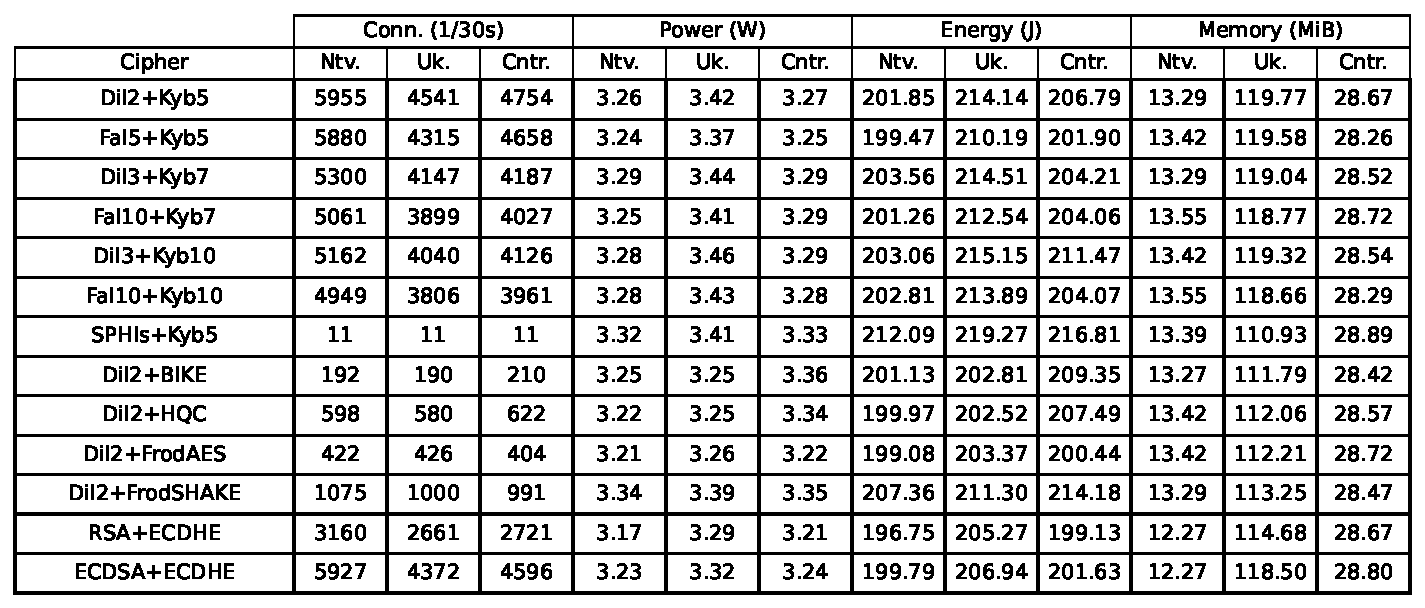
\includegraphics[width=1\textwidth]{resources/table_tls.pdf}
    \caption{Time, Power, Energy, and Memory consumption of Traditional and PQ TLS 1.3 Handshake.}
\end{figure}

\begin{figure}[h]
    \centering
	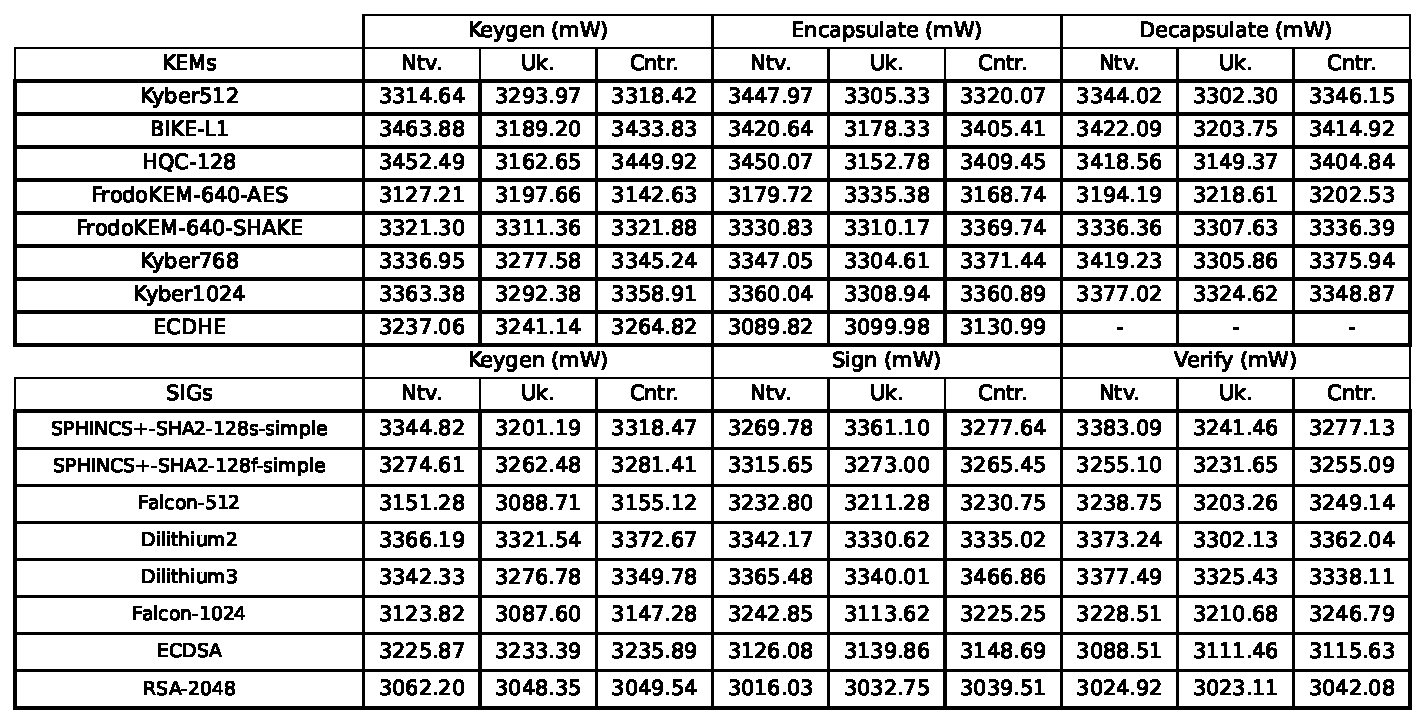
\includegraphics[width=1\textwidth]{resources/table_primitives_power.pdf}
    \caption{Power Consumption (mW) of Traditional and Post-quantum Primitives.}
\end{figure}

\begin{figure}[h]
    \centering
	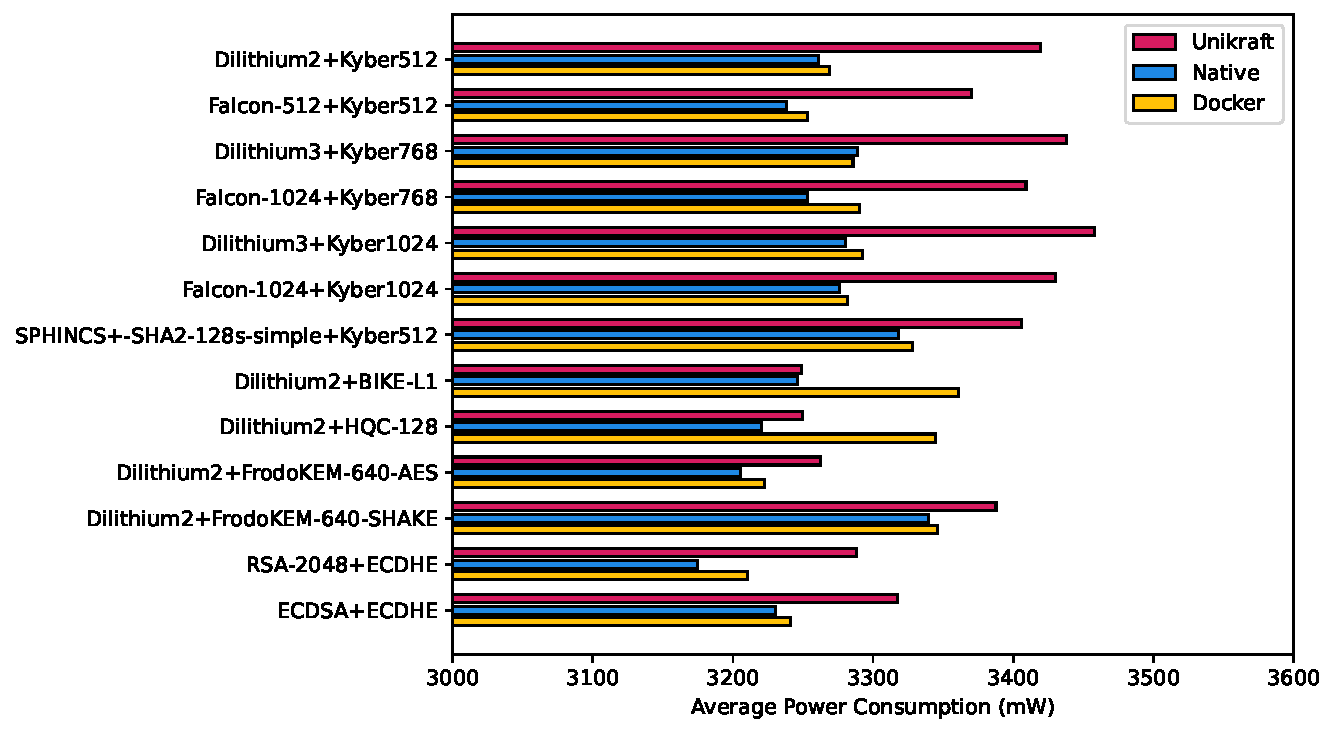
\includegraphics[width=1\textwidth]{resources/bar_tls_power.pdf}
    \caption{Power Consumption of Traditional and PQ TLS 1.3 handshakes.}
\end{figure}

\begin{figure}[h]
    \centering
	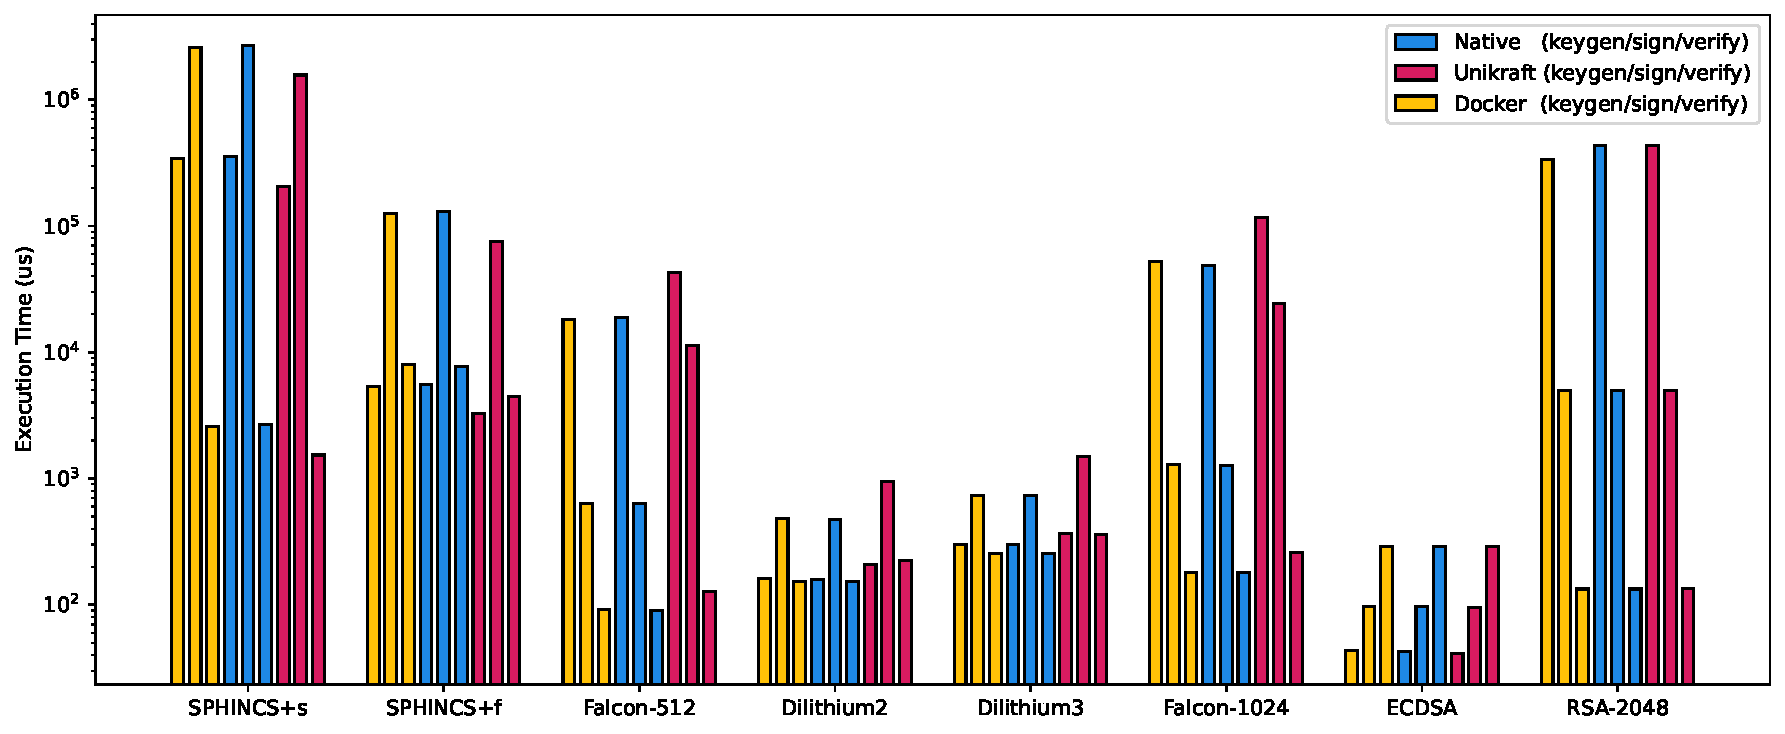
\includegraphics[width=1\textwidth]{resources/bar_sig_speed.pdf}
    \caption{Speed of Primitive Signature Algorithms.}
\end{figure}

\begin{figure}[h]
    \centering
	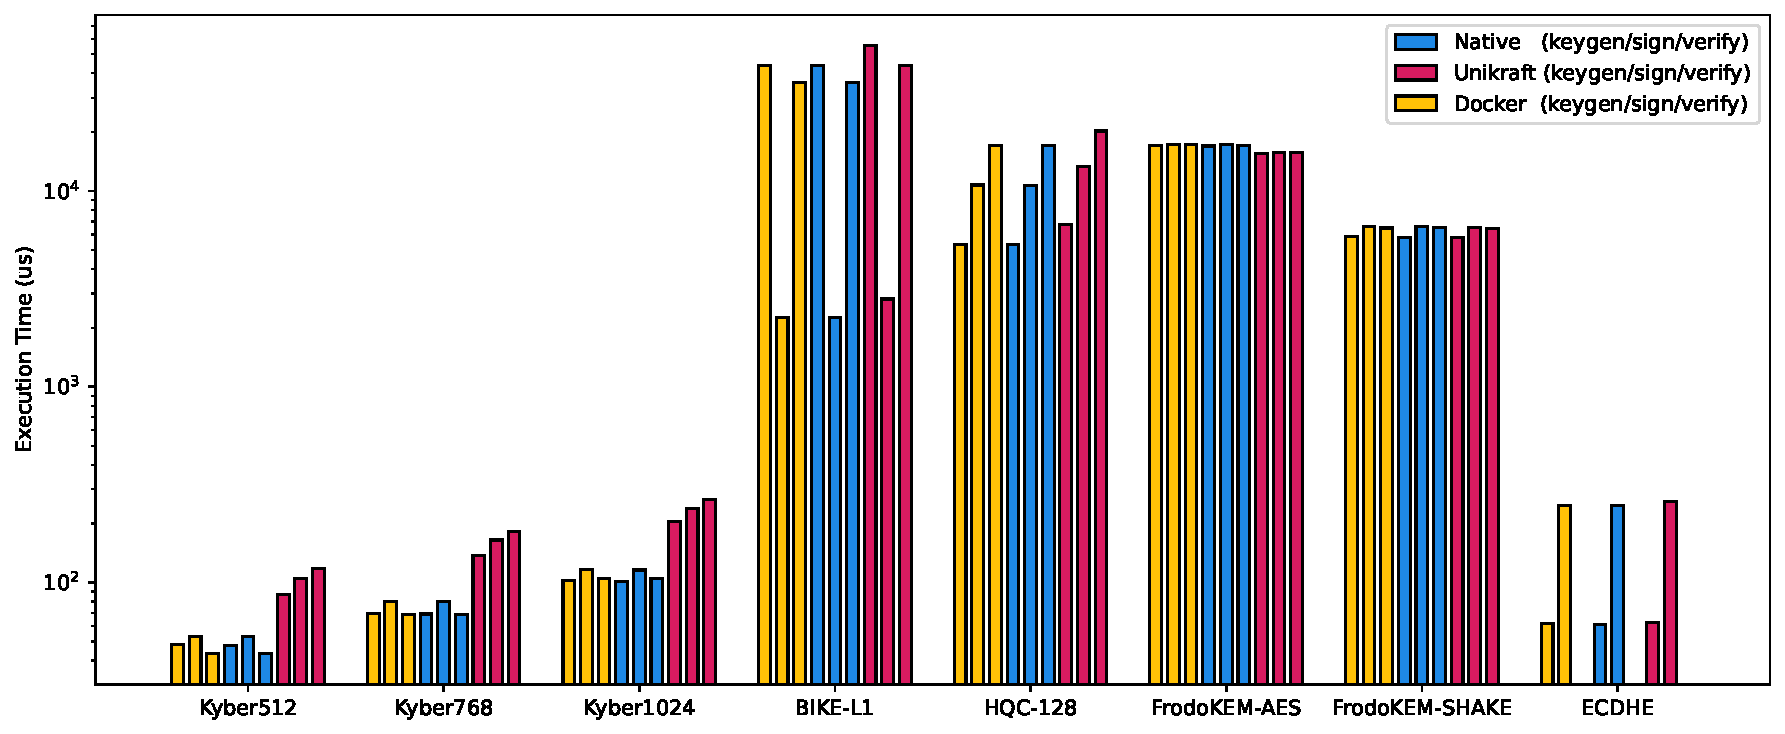
\includegraphics[width=1\textwidth]{resources/bar_kem_speed.pdf}
    \caption{Speed of Primitive KEM Algorithms.}
\end{figure}

% \section{Setup Images}

\begin{figure}[h]
    \centering
    \begin{subfigure}{0.45\textwidth}
        \centering
        \includegraphics[width=\textwidth]{resources/setup_img_01.png}
    \end{subfigure}\hfill
    \begin{subfigure}{0.45\textwidth}
        \centering
        \includegraphics[width=\textwidth]{resources/setup_img_02.png}
    \end{subfigure}
\end{figure}

\begin{figure}[h]
    \centering
    \begin{subfigure}{0.45\textwidth}
        \centering
        \includegraphics[width=\textwidth]{resources/setup_img_03.png}
    \end{subfigure}\hfill
    \begin{subfigure}{0.45\textwidth}
        \centering
        \includegraphics[width=\textwidth]{resources/setup_img_04.png}
    \end{subfigure}
\end{figure}

\end{document}
